\section{Experiments}
\label{sec:experiments}
\textbf{Method names.} Potential and Velocity denote potential-space and velocity-space spectral training, respectively. Both generate velocity by differentiating neural potentials; NKB predicts velocity directly. Laplacian is the numerical spectral baseline. Potential-FG and Potential-AL denote the finite-gauge and augmented-Lagrangian potential controls. The same names label all figures and tables.

We evaluate how spectral objectives, harmonic completion, and reduced dynamics shape a learned flow basis. A periodic vortex merger measures learned-basis autonomous accuracy and viscous decay. One-, two-, and three-hole domains test the circulation sector and the conditioning of its neural coordinates. A three-dimensional Metaball domain then connects spatial capacity to autonomous accuracy and coefficient-space cost (\docref{Table}{tab:experiment-map}).
\begin{table}[!htb]
\centering\small
\caption{{Validation goals and controlled comparisons.}}
\label{tab:experiment-map}
\setlength{\tabcolsep}{5pt}
\renewcommand{\arraystretch}{1.13}
\begin{tabular}{@{}>{\raggedright\arraybackslash}p{.14\linewidth}>{\raggedright\arraybackslash}p{.36\linewidth}>{\raggedright\arraybackslash}p{\dimexpr.50\linewidth-4\tabcolsep\relax}@{}}\toprule
Case & Comparison & {Validation}\\\midrule
Periodic & Learned spectral and kinematic bases; same-capacity Laplacian & {Neural eigenfluid and potential-space feasibility; autonomous accuracy and decay.}\\
Multi-hole & Random small-scale fields and large-scale vortices; fixed-budget allocation and lift conditioning & {Topology-aware circulation completion, energy capture and harmonic conditioning.}\\
Metaball & Velocity-basis capacity; full-grid and assembled coefficient operators & {3D feasibility, capacity-dependent representation and coefficient-space acceleration.}\\\bottomrule
\end{tabular}
\end{table}

{The field comparisons show the numerical ground-truth flow reference (Numerical GT), a same-capacity Laplacian basis, a potential-trained basis, and a velocity-trained basis. Let $u(t)$ be a reduced velocity and $u_{\rm GT}(t)$ the numerical reference at time $t$. Annotations give relative velocity error $e_u(t)=\|u(t)-u_{\rm GT}(t)\|_{L^2}/\|u_{\rm GT}(t)\|_{L^2}$, where $L^2$ is the spatial mass norm over the full assessment domain and plotted percentages are $100e_u$; we also write $e(t)=e_u(t)$. A subscript GT denotes a reference quantity; shared color scales preserve amplitude differences. \docref{Appendix}{app:protocol} gives discretizations and convergence checks. \docref{Figure}{fig:multihole-modes} compares the multiply connected modes, complemented by the periodic and three-dimensional atlases in \docref{Appendix}{app:modes}.}

A fixed-case adaptation of Neural Kinematic Bases {\citep{liu2025neural}} provides an additional direct-velocity comparison under the stated training budget and common Galerkin evolution (\docref{Appendix}{app:nkb}). Experiments are conducted on a workstation with an Intel Core i9-14900K CPU and an NVIDIA GeForce RTX 4080 SUPER GPU.

\subsection{Case 1: Periodic vortex merger}
\label{sec:case1}
The periodic domain admits an analytic Fourier basis and a mean-zero scalar gauge, providing a controlled setting for autonomous flow with learned spatial coordinates. The vortex pair has separation $d=1.35$, with $K=1024$ modes and a final simulation time $T=18\pi$. All methods project the same initial velocity with the full mass matrix and retain every basis coordinate during evolution. {The Laplacian (Fourier) basis supplies the same-capacity numerical control, following Laplacian Eigenfluids \citep{dewitt2012fluid}.}

\paragraph{Autonomous evolution.}
\docref{Figure}{fig:case1-field} shows the potential-trained seed-0 trajectory through $t=0,9\pi,18\pi$. \docref{Figure}{fig:case1-wide} measures velocity and vorticity errors, kinetic-energy decay, and enstrophy decay on the same case. The spatial basis is reused throughout the trajectory.
\begingroup
Both learned spectral objectives sustain sub-percent velocity error. Velocity learning gives the higher accuracy, while potential learning reduces training cost, matching the cost--accuracy tradeoff predicted by the objective analysis (\docref{Figure}{fig:case1-wide}; \docref{Table}{tab:runtime-training}). The potential and NKB trajectories have nearly identical synchronized integration times, yet the spectral span gives substantially smaller flow error (\docref{Table}{tab:runtime-2d-online}). Spectral organization therefore improves autonomous accuracy at comparable recurrent cost under this matched protocol. The absolute mean squared velocity error is reported in \docref{Table}{tab:case1}.
\par\endgroup
\begin{table}[!htb]\centering\small
\caption{Periodic vortex merger, $d=1.35$, $T=18\pi$, $K=1024$. Velocity mean squared error (MSE) averages squared velocity-component errors over all 241 saved $128^2$ observation-grid states. Learned entries then average three seeds. Relative errors are visualized in \docref{Figure}{fig:case1-wide}; training costs appear in \docref{Table}{tab:runtime-training}. NKB uses the 2000-update adaptation in \docref{Appendix}{app:nkb}.}
\label{tab:case1}
\begin{tabular}{lr}\toprule
Basis & Velocity MSE\\\midrule
Laplacian & $9.737\times10^{-10}$\\
Velocity & $8.882\times10^{-9}$\\
Potential & $1.619\times10^{-7}$\\
NKB & $2.823\times10^{-3}$\\
\bottomrule\end{tabular}\end{table}
\begin{figure}[!htb]
\centering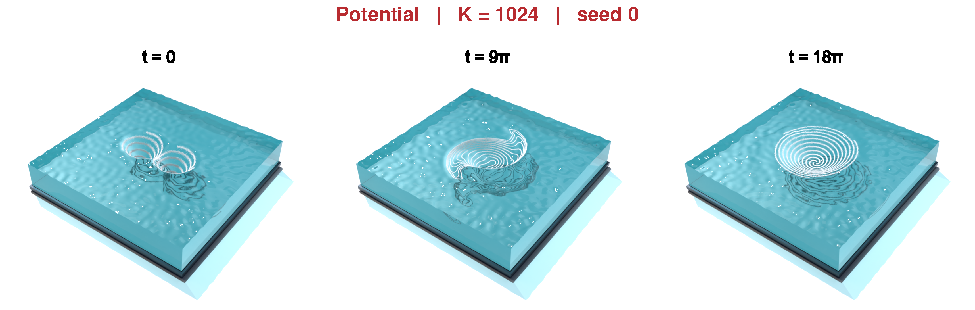
\includegraphics[width=\linewidth,height=.72\textheight,keepaspectratio]{unified_names_20261021_v1/case1_houdini_evolution.pdf}
\caption{\textbf{Potential: periodic vortex merger.} Panels show the $K=1024$, seed-0 Potential trajectory with vortex separation $d=1.35$, from left to right at $t=0,9\pi,18\pi$. Surface relief encodes smoothed vorticity magnitude on a common scale; white accents trace vortex structure. Height is a display coordinate for the two-dimensional flow.}
\label{fig:case1-field}
\end{figure}
\begin{figure}[!htb]
\centering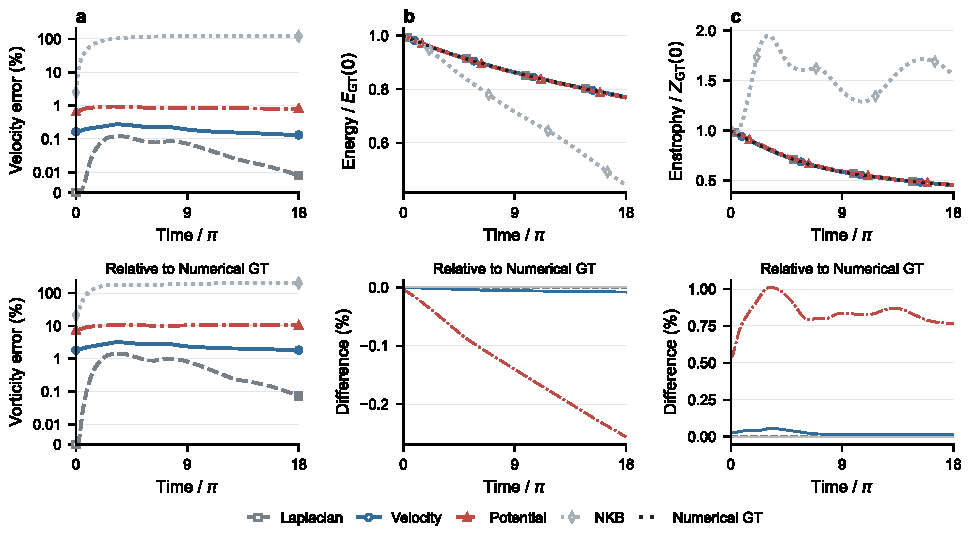
\includegraphics[width=\linewidth,height=.72\textheight,keepaspectratio]{unified_names_20261021_v1/case1_merger_diagnostics.pdf}
\caption{\textbf{Autonomous accuracy and decay in vortex merger.} All panels use $K=1024$, $d=1.35$, $T=18\pi$. (a) Relative velocity (top) and vorticity (bottom) errors against Numerical GT, normalized by the corresponding time-dependent observation-grid $L^2$ norm. Learned curves show three-seed means with one sample standard deviation (SD), on a symmetric-log scale with a linear interval below $0.01\%$. Open and filled markers indicate initial and final states. (b) Kinetic energy, $E=\frac12\langle|u|^2\rangle$. (c) Enstrophy, $Z=\frac12\langle\omega^2\rangle$, where $\omega=\partial_xu_y-\partial_yu_x$ is scalar vorticity, $u_x,u_y$ are velocity components, and $\langle\cdot\rangle$ denotes the spatial mean. {All five methods appear in the upper decay panels, using seed-0 learned trajectories and common initial GT normalization. Distinct line styles and sampled markers distinguish nearly overlapping curves. The lower panels of (b,c) show $100(E-E_{\rm GT})/E_{\rm GT}$ and $100(Z-Z_{\rm GT})/Z_{\rm GT}$ for Laplacian, velocity and potential bases.} Curves use all 241 saved $128^2$ states from $256^2$ operator quadrature and maximum step $0.005$.}
\label{fig:case1-wide}
\end{figure}



\subsection[Case 2: Multiply connected flow: energy compression and circulation]{Case 2: Multiply connected flow---energy compression and circulation}
\label{sec:case2}
Each obstacle introduces an independent circulation coordinate. We consider two random flow ensembles: streamfunctions with many small-scale vortical structures, and combinations of a few smooth, large-scale vortices. Together they test energy compression, harmonic completion, and lift conditioning. The small-scale random-field comparison uses total $K=1024$ throughout: $P_K$ and $P_{K-h}+H_h$ exchange positive and harmonic coordinates within the same state budget.

\paragraph{Energy captured per reduced coordinate.}
\begingroup
We sample streamfunctions in physical space from Gaussian lattice values and a quintic spline, then condition each draw to impermeability and zero boundary vorticity before analytic differentiation. Boundary constants are derived from the same draw, so its vortical and circulation content arise together. Frozen seeds $[20260928,\text{topology index},\text{field index}]$ define 20 reproducible fields per topology; indices 0 and 1 supply the six-field all-method dynamic comparison. \docref{Appendix}{app:random-streamfunction} specifies the generator, conditioning, and reference construction.
\par\endgroup


\begingroup
Let $W$ be the positive assessment quadrature matrix, with $\|v\|_W^2=v^{\top}Wv$ for sampled velocity $v$, and let $u_K=Uc_0$ be the full-mass projection of $u_0$, with initial coefficient vector $c_0=c(0)$. The captured kinetic-energy fraction is $\eta=\|u_K\|_W^2/\|u_0\|_W^2$. Potential bases capture more initial kinetic energy than equal-capacity Laplacian controls across all three topologies, with the largest gains in the two- and three-hole domains, while compressing the reference state by roughly three orders of magnitude (\docref{Figure}{fig:random-k1024-energy}). Most energy in these small-scale random fields lies in the vortical sector, represented by the spectrally ordered $P$ modes. Harmonic coordinates lift independent obstacle-boundary constants into circulation-carrying velocities \citep{arnold2006finite,liu2015model}. At fixed $K$, their added harmonic energy competes with the energy of the $h$ displaced positive modes. This energy allocation favors positive coordinates for the small-scale ensemble, while harmonic coordinates provide its independent circulation sector (\docref{Appendix}{app:random-streamfunction}).
\par\endgroup




\begin{figure}[!htb]\centering
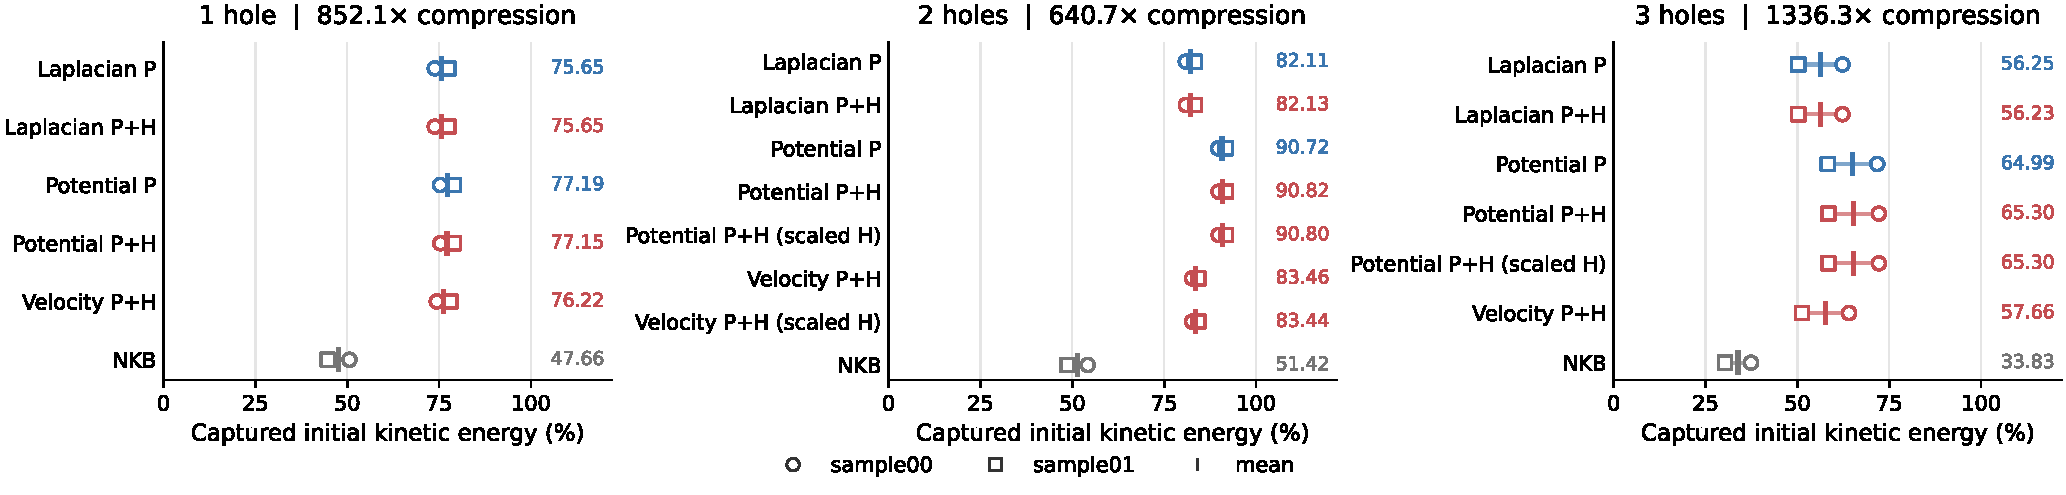
\includegraphics[width=\linewidth,height=.72\textheight,keepaspectratio]{unified_names_20261021_v1/random_k1024_initial_energy_capture.pdf}
\caption{Initial energy captured by the original $K=1024$ representations. Circles and squares denote the two predetermined physical fields in each topology; vertical ticks denote their mean. The annotations give mean captured-energy percentages and state-coordinate compression $N_{\rm ref}/K$, where $N_{\rm ref}$ is the number of independent coordinates of the reference state. The complete set of learned branches, raw/scaled harmonic coordinates, numerical controls, and NKBs use the same analytic initial fields.}
\label{fig:random-k1024-energy}
\end{figure}

\paragraph{Autonomous dynamics at the same capacity.}
\begingroup
Each representation evolves from its analytic-field projection using the full Galerkin operators, $\nu=1/750$, and $T=1$. The Potential P span combines higher initial energy capture with lower final trajectory error than the same-capacity Laplacian P control in every topology. \docref{Table}{tab:completion-improvement} quantifies the paired effects of coordinate allocation on energy capture and trajectory accuracy. The nonlinear evolution couples these coordinates within the retained span. With $e_P,e_{PH}$ and $\eta_P,\eta_{PH}$ denoting the errors and energy fractions under the two allocations, its gains are $\Delta e=e_P-e_{PH}$ and $\Delta\eta=\eta_{PH}-\eta_P$, with positive values denoting improvement. \docref{Appendix}{app:random-k1024-six} gives the full method--field curves, reference checks, energy histories, and circulation diagnostics; \docref{Appendix}{app:random-streamfunction} provides the broader numerical capacity and low-dimensional allocation studies.
\par\endgroup
\begingroup
\begin{table}[!htb]\centering\small
\caption{Paired changes under harmonic allocation on the six qualified random fields at total $K=1024$. Each entry averages the two fixed fields in its topology. Initial capture $\eta$ uses the analytic-target full-mass projection; final velocity error uses the qualified numerical trajectory. Gains are $\Delta\eta=\eta_{PH}-\eta_P$ and $\Delta e(1)=e_P(1)-e_{PH}(1)$ in percentage points, so positive values favor completion. Absolute capture and trajectories are shown in \docref{Figures}{fig:random-k1024-energy} and~\ref{fig:random-k1024-errors}.}
\label{tab:completion-improvement}
\setlength{\tabcolsep}{4pt}
\begin{tabular}{rlrr}\toprule
Holes & Basis & $\Delta\eta$ & $\Delta e(1)$\\\midrule
1 & Laplacian & +0.004 & +0.020\\
1 & Potential & -0.045 & +0.092\\
2 & Laplacian & +0.018 & +0.087\\
2 & Potential & +0.102 & -0.243\\
3 & Laplacian & -0.014 & +0.021\\
3 & Potential & +0.305 & +0.942\\
\bottomrule\end{tabular}\end{table}
\par\endgroup



\paragraph{Completion and conditioning in random large-vortex flows.}
\begingroup
We randomly construct flows from a few smooth, large-scale vortices, with random locations, signs, and strengths. These flows combine local vorticity with motion around the obstacles. At $K=32$, harmonic completion consistently lowers final error across all three obstacle configurations and brings the learned completed bases close to the numerical completed controls (\docref{Table}{tab:prescribed32-summary}). The boundary lifts make the independent circulation component accessible within a fixed-size reduced state. The two ensembles thus expose complementary demands on the basis: small-scale random fields emphasize vortical energy capture, while random large-vortex flows make topological completion and lift conditioning visible.
\par\endgroup


{At $K=1024$, raw/scaled pairs share the positive checkpoint, boundary traces, Dirichlet objective, initialization, and training budget. Scaling substantially lowers the multi-hole trajectory errors (\docref{Figure}{fig:case2-ablation}), whereas changing the spectral objective in the raw two-hole control has little effect. The paired comparison identifies harmonic-lift conditioning as the main source of this improvement. \docref{Table}{tab:case2} gives the corresponding positive-only controls.}

\begin{table}[!htb]
\centering\small
\caption{Positive-only controls for the random large-vortex ensemble: final relative velocity error (\%), total $K=1024$, $T=1$, averaged over 20 initial states. Learned positive modes use potential training, seed 1. Completed bases and raw/scaled lift comparisons are visualized in \docref{Figure}{fig:case2-ablation}.}
\label{tab:case2}
\begin{tabular}{rrr}\toprule
Holes & Numerical $P$ & Learned $P$\\\midrule
1 &32.542&32.124\\
2 &34.197&33.963\\
3 &36.685&36.707\\\bottomrule
\end{tabular}
\end{table}
{Once the harmonic fields are consistently conditioned, potential and velocity learning produce similar trajectory errors. \docref{Figure}{fig:case2-field} shows the resulting flow, and \docref{Appendix}{app:fields} gives the matched-objective and conditioning comparisons.}

\begin{figure}[!htb]
\centering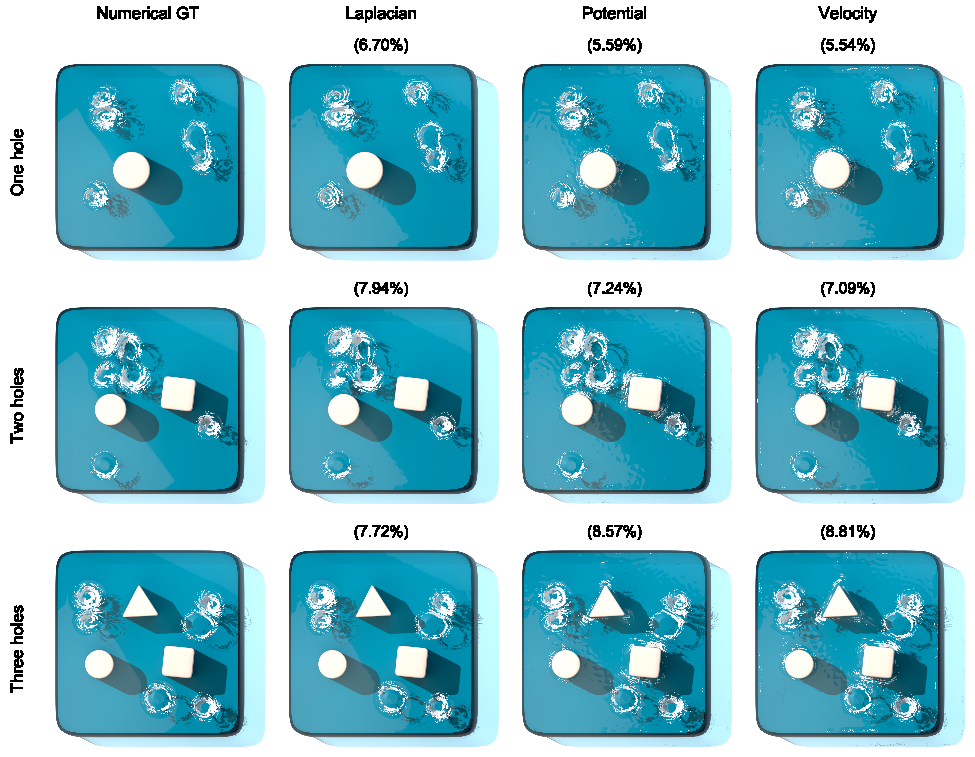
\includegraphics[width=\linewidth,height=.72\textheight,keepaspectratio]{unified_names_20261021_v1/case2_k1024_fourway_houdini.pdf}
\caption{\textbf{Random large-vortex flow at $K=1024$.} Rows: one-, two-, and three-hole domains. Columns: numerical reference, Laplacian, potential- and velocity-trained bases at $t=1$, seed 1, state 00. Reduced bases have $1024-h$ positive and $h$ harmonic coordinates; the learned objectives share raw $H_1$ and scaled $H_2,H_3$. Errors use the common level-2 reference. Overhead views share height and foam mappings within each geometry (\docref{Appendix}{app:fields}).}
\label{fig:case2-field}
\end{figure}

\begingroup
\paragraph{Topology-dependent spectral modes.}
\docref{Figure}{fig:multihole-modes} compares the first eight positive modes of the Laplacian and both learned constructions across three obstacle configurations. The aligned panels show each basis's spatial structure and ordering; independent harmonic coordinates complete the span.
\par\endgroup


\begin{figure}[!htb]
\centering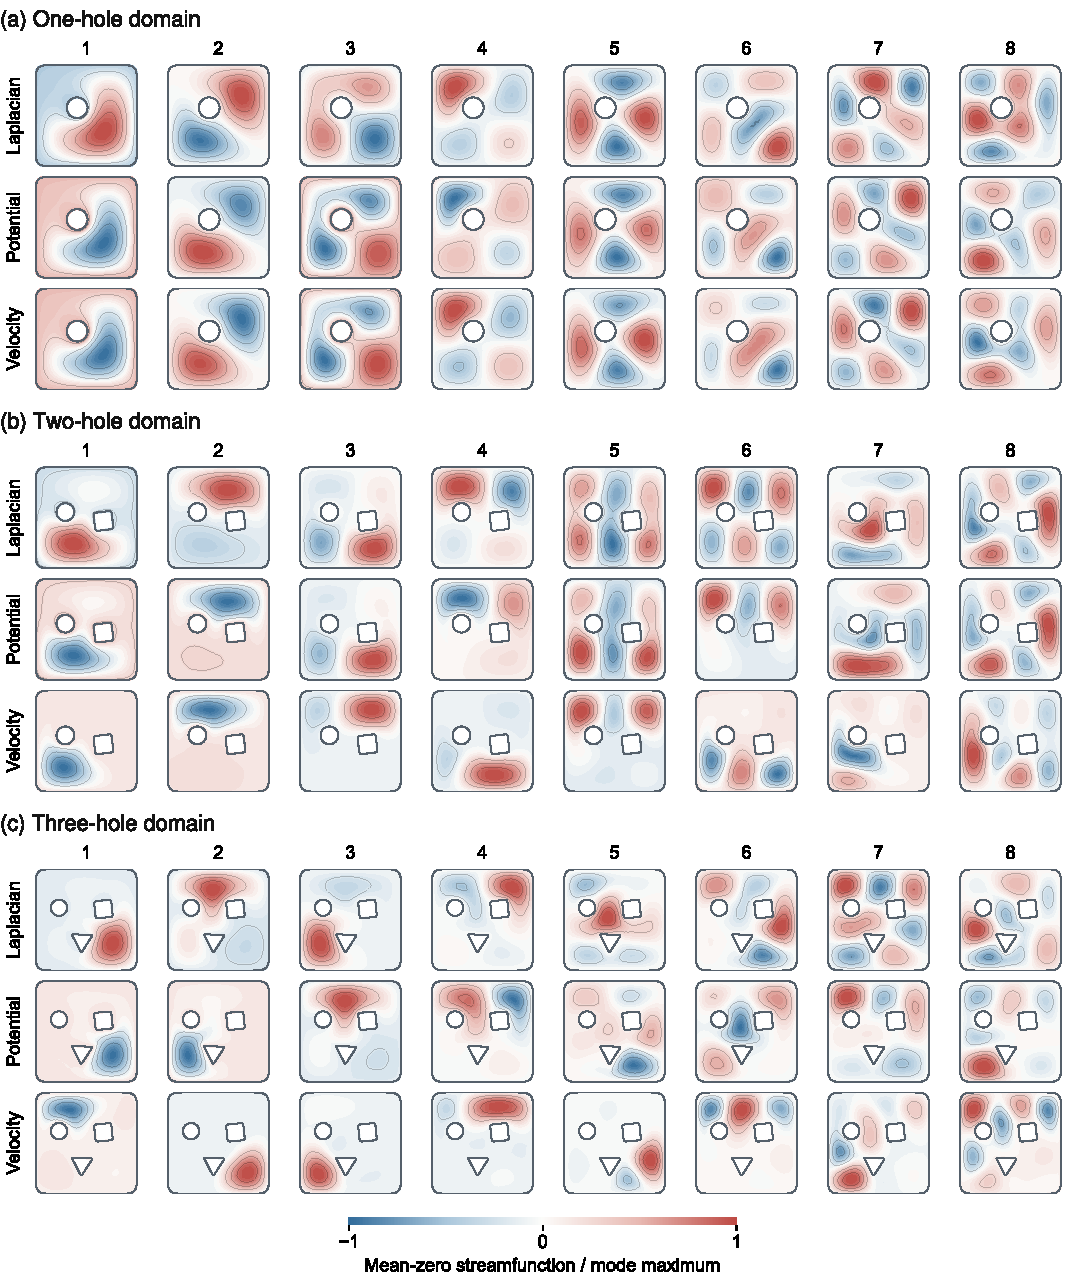
\includegraphics[width=\linewidth,height=.72\textheight,keepaspectratio]{unified_names_20261021_v1/case2_multihole_modes.pdf}
\caption{\textbf{Positive spectral modes across obstacle topologies.} Panels (a--c) show one-, two-, and three-hole domains. Within each panel, rows compare Laplacian, potential-trained, and velocity-trained fields; columns show modes 1--8. Learned fields follow the positive-mode selection order in the total-$32$ continuous piecewise-linear finite-element (P1) basis, whose $h$ harmonic coordinates are separate. The shared color scale shows area-centered streamfunction divided by its per-mode maximum magnitude. Signs and rotations within repeated eigenspaces preserve the span.}
\label{fig:multihole-modes}\end{figure}

\subsection[Case 3: 3D Metaball: representation and autonomous evolution]{Case 3: 3D Metaball---representation and autonomous evolution}
\label{sec:case3}
The three-dimensional domain tests how a learned span supports autonomous dynamics. We separate the error due to spatial representation from the error in coefficient evolution, then measure the cost of evaluating the same reduced generator entirely in coefficient space.

\paragraph{Autonomous flow at 1024 modes.}
{\docref{Figure}{fig:case3-field} compares a velocity-trained $K=1024$ basis with same-capacity Laplacian and NKB bases against the common independent $128^3$ normal-penalty Navier--Stokes (NS) reference. All three evolve autonomously from full-mass projections of the same initial field. Eigenfluid and Laplacian begin with comparable reconstruction quality and develop similar relative errors during autonomous evolution. The vector-error panels in \docref{Figure}{fig:case3-field} also highlight similar regions of elevated error. Their agreement in error magnitude and spatial structure identifies the shared role of truncated Galerkin dynamics. Both methods compress the flow into the same number of coordinates, with nonlinear interactions resolved within that span. This correspondence connects the learned continuous basis to the established spectral ROM behavior at the same compression level. \docref{Figure}{fig:case3-capacity} examines the joint contributions of spatial capacity and coefficient dynamics.}
\begin{figure}[!htb]
\centering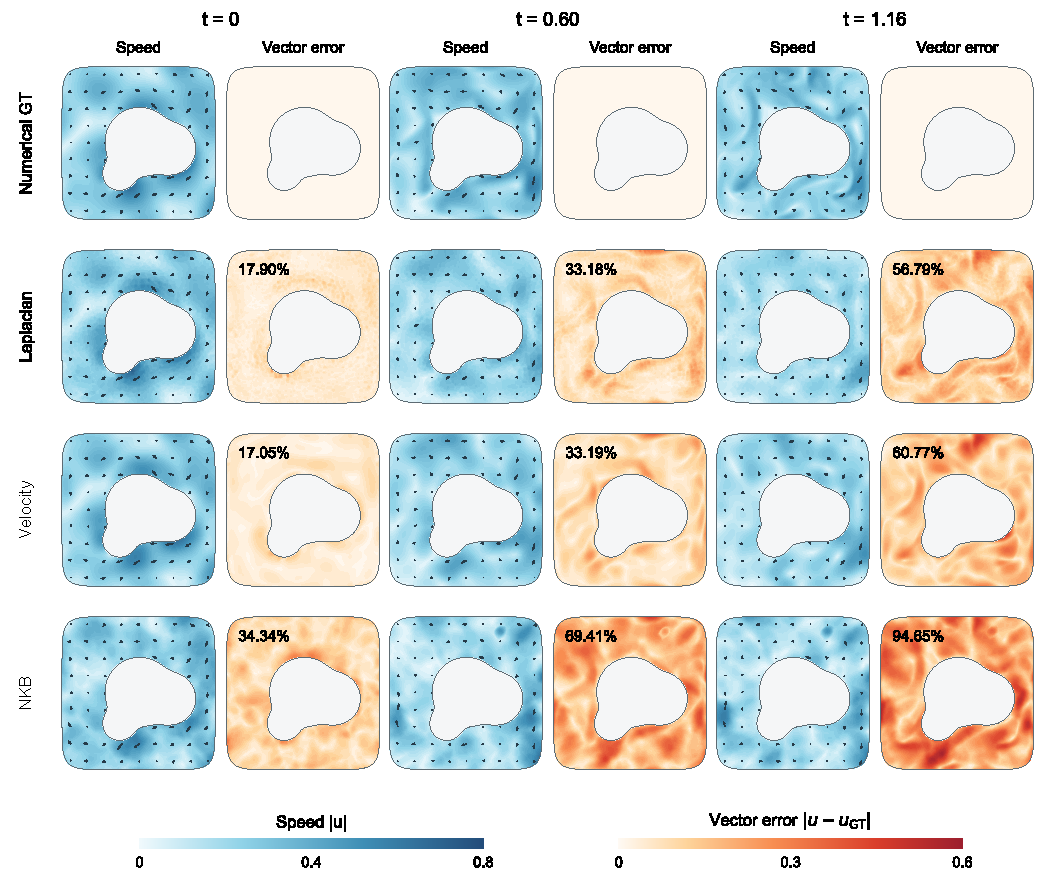
\includegraphics[width=\linewidth,height=.72\textheight,keepaspectratio]{unified_names_20261021_v1/case3_k1024_comparison.pdf}
\caption{\textbf{Three-dimensional autonomous flow at $K=1024$.} Rows show Numerical GT, Laplacian, Velocity, and NKB; columns show $t=0,0.60,1.16$. Each time pairs speed $|u|$ (blue) with pointwise vector error $|u-u_{\rm GT}|$ (orange--red) on the offset $z=0.31640625$ slice, which exposes the fused Metaball silhouette. Filled contours interpolate the saved nodal values and are clipped to the original geometry's smooth boundary. Speed, error, and in-plane arrow lengths use separate fixed scales across all methods and times. Percentages in the upper-left corner of the vector-error panels denote full-volume relative velocity error, evaluated on all 1,599,754 fluid nodes. Here $\Delta t$ is the integration time step; ROM trajectories use $\Delta t=0.000625$ and the common NS reference uses $\Delta t=0.0025$.}
\label{fig:case3-field}
\end{figure}

\paragraph{Spatial capacity.}
\begingroup
Increasing capacity improves both initial reconstruction and autonomous accuracy under the same training budget, full-volume reference, and assessment times (\docref{Figure}{fig:case3-capacity}). At $K=1024$, the learned velocity span has lower initial projection error than the Laplacian control. \docref{Appendix}{app:3d-high-capacity} gives the detailed projection and training-cost comparison.
\par\endgroup



\paragraph{Representation of randomized 3D large-eddy fields.}
Figure~\ref{fig:case3-Pot-capacity} compares the frozen Metaball spans on 20 independently randomized large-eddy initial states. A case-local Philox stream draws 96 independent standard-Gaussian sine and cosine coefficients for a three-component vector potential over 16 representatives of the integer wavevector pairs $\pm\boldsymbol{k}$ with $1\leq\|\boldsymbol{k}\|\leq2$. Coefficients are scaled by $1/\|\boldsymbol{k}\|$; the raw potential wavelengths range from $0.5$ to $1$ unit-domain length. The analytic curl follows the common $128^3$ Metaball incompressibility projection and boundary conditioning, RMS normalization to $0.32$, and four warm-up substeps. Each frozen basis projects the same states using the full physical mass matrix, all 1,599,754 fluid nodes, and all $K$ retained coordinates. Errors decrease with capacity; at $K=256$, mean relative velocity errors are Laplacian $26.51102\pm3.94584\%$, Velocity $31.26405\pm5.95889\%$, Potential $26.10521\pm3.97608\%$, and NKB $56.03645\pm2.70518\%$ (mean $\pm$ sample standard deviation). At $K=512$, Potential gives $23.73323\pm3.99279\%$, compared with Laplacian $23.90729\pm4.04593\%$, with lower Potential error in 15 of the same 20 states. This paired assessment measures representation of independently sampled large eddies with each training checkpoint held fixed; the autonomous-flow study evaluates evolution on its trajectory initial condition. Assessment states are separate from basis training and selection, and NKB uses geometry alone. The $K=1024$ results for Velocity, Laplacian, and NKB are reported separately in Appendix~\ref{app:randomfield-values}. At $K=512$, Potential training takes 140.20 hours for 2000 updates, compared with 3.99 hours for Velocity, while its mean random-field error is only 0.17 percentage points below Laplacian. At this three-dimensional scale, that small gain over the numerical basis does not justify the Potential training cost. We therefore favor Velocity when a learned high-capacity basis is required and Laplacian for fixed-domain reconstruction. Appendix~\ref{app:old-Pot} documents the Potential-FG and Potential-AL configurations; Appendix~\ref{app:Pot-cost} reports preparation costs.
\begin{figure}[!htb]
\centering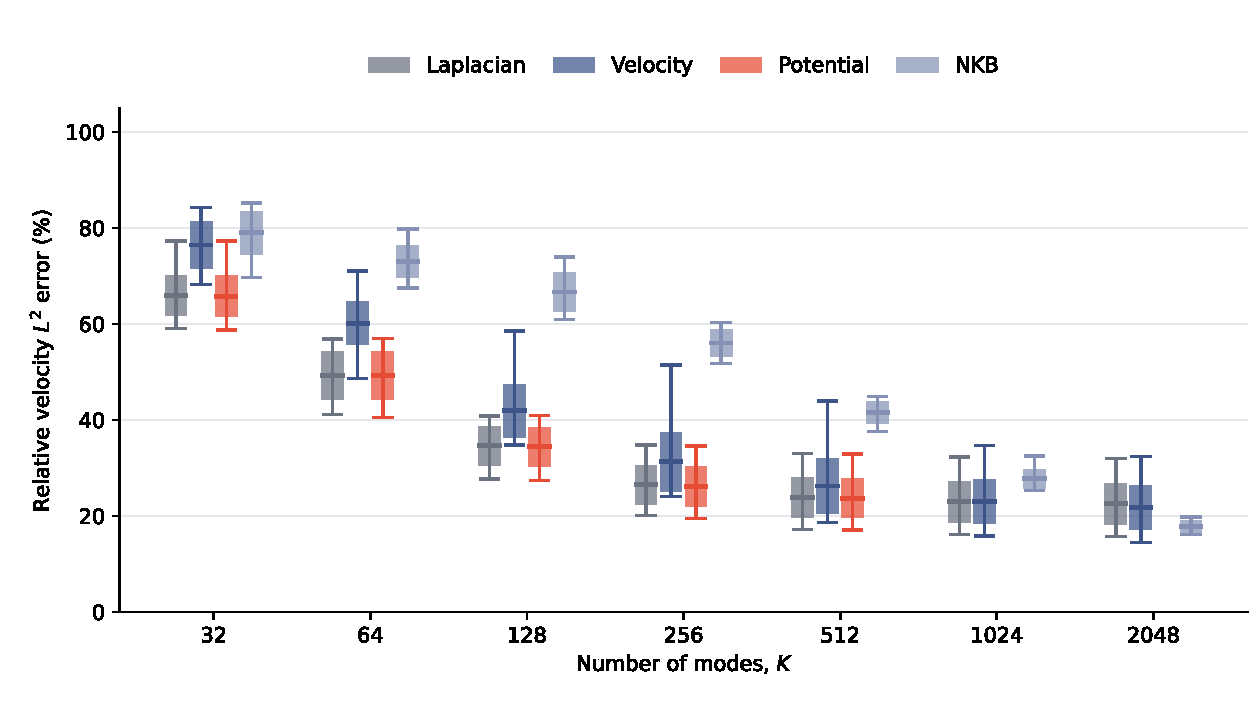
\includegraphics[width=\linewidth,height=.78\textheight,keepaspectratio]{unified_names_20261021_v1/case3_large_eddy20_method_names_20261021_v1.pdf}
\caption{\textbf{Representation of independently randomized large-eddy fields.} Relative velocity $L^2$ errors on the same 20 paired initial states generated by independent Gaussian vector-potential Fourier coefficients and common Metaball physical conditioning. The 20 method--capacity groups contain 400 model--field measurements. Solid rectangles span mean $\pm$ sample standard deviation ($n=20$, $\mathrm{ddof}=1$); whisker caps show the observed minimum and maximum. Each frozen basis uses all $K$ retained modes and all 1,599,754 fluid nodes in the full-mass representation comparison. All four methods are compared through $K=512$; the $K=1024$ comparison is given in Appendix~\ref{app:randomfield-values}. Horizontal offsets separate the methods at each capacity.}
\label{fig:case3-Pot-capacity}
\end{figure}

\paragraph{Separating the two error sources.}
{Projection onto each frozen span separates autonomous error into orthogonal representation and in-span coefficient terms (\doceqref{eq:error-split}). The extended decomposition shows the same pattern through 1024 modes: a richer span lowers the best-projection error, while the coefficient term remains nearly unchanged at the upper capacities (\docref{Table}{tab:3d-error-attribution}). Spatial refinement and coefficient evolution thus control complementary parts of the reduced model. The decomposition makes the representation gain explicit and connects the common evolution pattern to the retained-coordinate dynamics.}
\begin{figure}[!htb]
\centering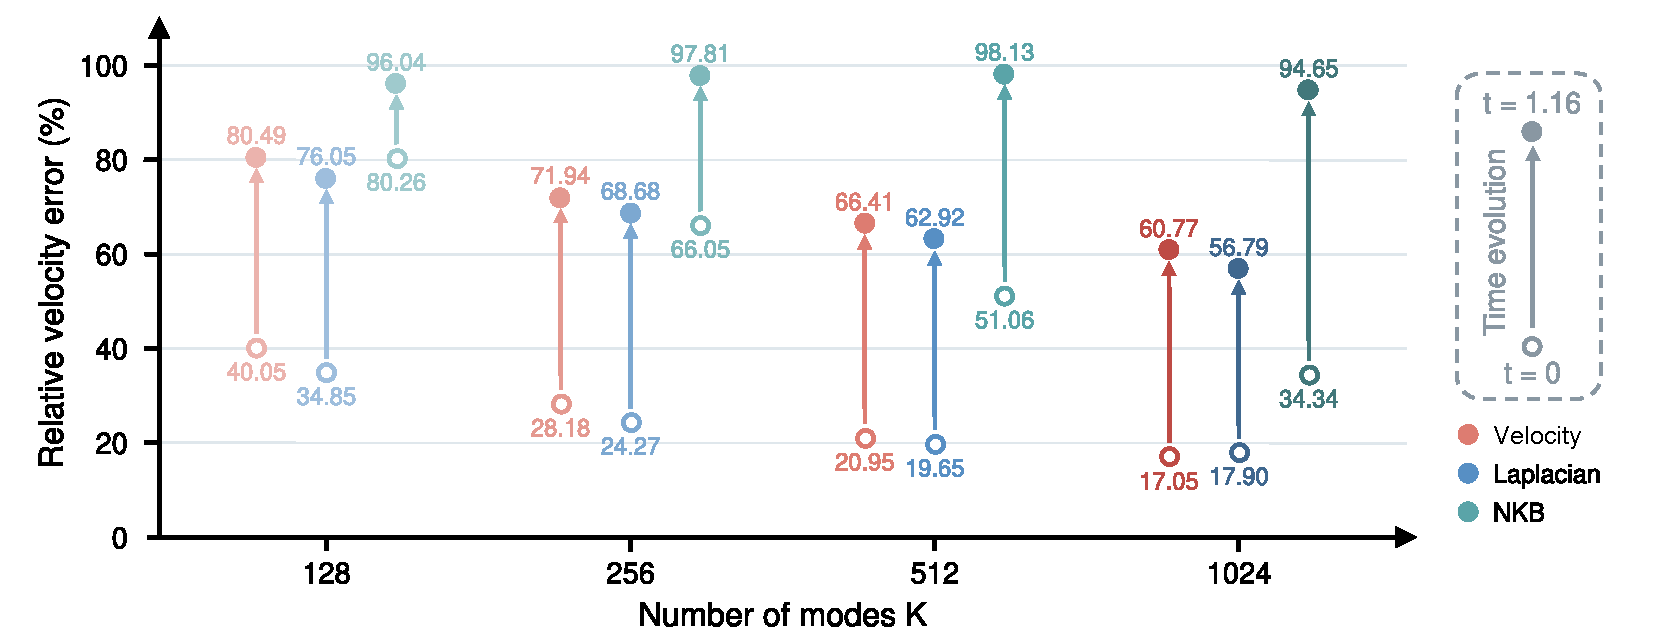
\includegraphics[width=\linewidth,height=.72\textheight,keepaspectratio]{unified_names_20261021_v1/case3_capacity_to1024.pdf}
\caption{\textbf{Spatial capacity and autonomous accuracy through 1024 modes.} Initial full-mass projection error (open circles, $t=0$) and final autonomous error (filled circles, $T=1.16$) for $K=128,256,512,1024$. Within each capacity, Velocity, Laplacian, and NKB bases are offset from left to right for readability; color identifies the basis and darkens with increasing capacity. Arrows connect the two assessment times. All errors are percentages, evaluated against the same full-volume reference using all trained coordinates. Each trajectory has 30 stored states through $T=1.16$, with ROM step $\Delta t=0.000625$ and common NS reference step $\Delta t=0.0025$. Training costs are listed in \docref{Table}{tab:runtime-training}. The error decomposition is specified in \docref{Appendix}{app:3d-error}.}
\label{fig:case3-capacity}
\end{figure}

\paragraph{Exact coefficient-space execution.}
\begingroup
Preassembling the full quadratic Galerkin operator moves spatial evaluation out of recurrent time stepping. The resulting integration is faster than the matched-step NS control at both tested capacities, with assembled and direct reduced right-hand sides agreeing to numerical precision. This acceleration comes from executing the same reduced generator in coefficient space. \docref{Table}{tab:coefficient-capacity} reports timings and one-time assembly costs; \docref{Figure}{fig:coefficient-capacity} shows the associated flow errors. Repeated initial-condition queries reuse that assembly, motivating the \hyperref[sec:inference-cost]{amortization analysis below}.
\par\endgroup

\paragraph{Continuous reconstruction across query domains.}
{The same frozen neural map can be evaluated at held-out points and on three unseen domains. \docref{Appendix}{app:unseen-geometry} reports these reconstruction measurements together with target-specific numerical controls. This assessment complements the capacity study by examining how the continuous coordinates respond to changes in query location and geometry.}




\subsection{Continuous basis queries and amortized inference}
\label{sec:inference-cost}
The learned object is the map $(\mathbf x,\mathbf g)\mapsto U_\theta(\mathbf x;\mathbf g)$ from spatial coordinates and geometry parameters to a vector-valued basis. Once trained, this map supplies basis values and analytic spatial derivatives at newly requested locations without repeating variational optimization or solving a new eigenproblem. It supports arbitrarily dense spatial resampling: there is no fixed output lattice or discrete set of admissible query points. For a geometry-conditioned model, geometry parameters can likewise be queried continuously within its learned family. The three-dimensional capacity experiment uses a fixed-domain checkpoint; the continuous geometry-family construction is exercised in the planar cases.

\paragraph{Online latency and numerical comparison.}
\begingroup
The map supplies spatial fields once a geometry is selected; operator assembly then prepares their recurrent coefficient dynamics. Synchronized measurements give mean RK4 update times of 3.79 ms at $K=512$ and 26.18 ms at $K=1024$, with field reconstruction charged at requested outputs. \docref{Figure}{fig:coefficient-capacity} places integration costs alongside flow errors. This cost separation makes reuse explicit: trajectories on one geometry share the basis and assembled operators, while initial projection and selected field outputs belong to each query.
\par\endgroup

\paragraph{When repeated inference recovers training cost.}
For $n$ trajectories on one geometry, let $T_{\rm train}$ denote training, $T_{\rm off}$ the reusable preparation cost, and $T_{\rm ROM},T_{\rm NS}$ the per-trajectory integration costs. The smallest integration-only break-even count $n_\star$ is given below, with $\lceil\cdot\rceil$ denoting rounding up to an integer:
\begin{equation}
n_\star=\left\lceil\frac{T_{\rm train}+T_{\rm off}}{T_{\rm NS}-T_{\rm ROM}}\right\rceil,
\qquad T_{\rm NS}>T_{\rm ROM}.
\label{eq:inference-break-even}
\end{equation}
{Repeated initial-condition queries amortize both training and reusable operator preparation. \docref{Table}{tab:inference-amortization} gives the counts and exact timer boundaries. Projection and requested field output enter the per-query cost when included in the workload. For a parameterized family, training is shared across geometry queries, while each geometry's basis generation and operator preparation are charged to that query (\docref{Appendix}{app:inference-amortization}).}

